\documentclass[aspectratio=169,10pt]{beamer}
% Shared Beamer setup for Fall 2026 course slides.
% Clean Cal Poly-inspired theme: no custom class files or uncommon packages.
\mode<presentation>{
  \usetheme{default}
  \usefonttheme{professionalfonts}
}

\definecolor{CalPolyGreen}{HTML}{154734}
\definecolor{CalPolyGold}{HTML}{BD8B13}
\definecolor{CalPolySage}{HTML}{7FA28F}
\definecolor{CalPolyMint}{HTML}{DDF1E7}
\definecolor{CalPolySand}{HTML}{A29F86}
\definecolor{CalPolyBeige}{HTML}{EFEEDE}
\definecolor{DeckInk}{HTML}{1F2933}
\definecolor{DeckMuted}{HTML}{5F6B7A}
\definecolor{DeckSoft}{HTML}{F7F7F5}

\setbeamersize{text margin left=0.55in,text margin right=0.55in}
\setbeamercolor{normal text}{fg=DeckInk,bg=white}
\setbeamercolor{structure}{fg=CalPolyGreen}
\setbeamercolor{title}{fg=white}
\setbeamercolor{frametitle}{fg=CalPolyGreen,bg=white}
\setbeamercolor{block title}{bg=CalPolySage,fg=white}
\setbeamercolor{block body}{bg=CalPolyMint,fg=black}
\setbeamercolor{alerted text}{fg=CalPolyGold}

\setbeamerfont{title}{size=\Huge,series=\bfseries}
\setbeamerfont{frametitle}{size=\Large,series=\bfseries}
\setbeamerfont{block title}{size=\normalsize,series=\bfseries}

\setbeamertemplate{navigation symbols}{}
\setbeamertemplate{itemize item}{\color{CalPolyGold}$\blacktriangleright$}
\setbeamertemplate{itemize subitem}{\color{CalPolyGreen}$\bullet$}
\setbeamertemplate{footline}{
  \hfill{\color{DeckMuted}\scriptsize\insertframenumber/\inserttotalframenumber}
  \hspace{0.18in}\vspace{0.12in}
}
\setbeamertemplate{frametitle}{
  \vspace{0.18in}
  \hspace{0.02in}\insertframetitle\par
  \vspace{0.08in}
  \noindent\makebox[\linewidth][l]{%
    {\color{CalPolyGold}\rule{0.55in}{2pt}}%
    {\color{CalPolyGreen}\rule{\dimexpr\linewidth-0.55in\relax}{2pt}}%
  }
}

\newcommand{\CourseNumber}{Course}
\newcommand{\CourseTitle}{Course Title}
\newcommand{\LectureNumber}{0}
\newcommand{\LectureTitle}{Lecture Title}
\newcommand{\LectureDate}{Date}
\newcommand{\CourseUnit}{Unit}

\newcommand{\coursenumber}[1]{\renewcommand{\CourseNumber}{#1}}
\newcommand{\coursetitle}[1]{\renewcommand{\CourseTitle}{#1}}
\newcommand{\lecturenumber}[1]{\renewcommand{\LectureNumber}{#1}}
\newcommand{\lecturetitle}[1]{\renewcommand{\LectureTitle}{#1}}
\newcommand{\lecturedate}[1]{\renewcommand{\LectureDate}{#1}}
\newcommand{\courseunit}[1]{\renewcommand{\CourseUnit}{#1}}

\author{Kirk Duran}
\institute{California Polytechnic State University, San Luis Obispo}
\date{\LectureDate}

\newcommand{\makedecktitle}{
  \begingroup
  \setbeamercolor{background canvas}{bg=CalPolyGreen}
  \begin{frame}[plain]
    \vfill
    \begin{center}
      {\usebeamerfont{title}\color{white}\LectureTitle\par}
      \vspace{0.18in}
      {\Large\color{white}Lecture \LectureNumber\par}
    \end{center}
    \vfill
    \noindent{\color{white}\rule{\linewidth}{1.2pt}}\par
    \vspace{0.08in}
    \noindent\colorbox{CalPolyGold}{\makebox[0.24\linewidth][c]{\color{white}\Large\CourseNumber}}
    \hspace{0.12in}{\color{white}\Large Kirk Duran}
  \end{frame}
  \endgroup
}

\newenvironment{keyidea}{\begin{block}{Key idea}}{\end{block}}
\newenvironment{activity}{\begin{block}{In class}}{\end{block}}
\newenvironment{cpdefinition}{\begin{block}{Definition}}{\end{block}}
\newenvironment{exampleblockcp}{
  \begingroup
  \setbeamercolor{block title}{bg=CalPolySand,fg=white}
  \setbeamercolor{block body}{bg=CalPolyBeige,fg=black}
  \begin{block}{Example}
}{
  \end{block}
  \endgroup
}

\newcommand{\imageplaceholder}[2][0.3in]{%
  \noindent\makebox[\linewidth][c]{%
    \fcolorbox{CalPolySage}{CalPolyBeige}{%
      \parbox[c][#1][c]{0.86\linewidth}{%
        \centering
        {\color{DeckMuted}\scriptsize Image placeholder: }%
        {\color{DeckInk}\scriptsize\ttfamily\detokenize{#2}}%
      }%
    }%
  }%
}

\newcommand{\sectionframe}[1]{
  \begingroup
  \setbeamercolor{background canvas}{bg=CalPolyGreen}
  \begin{frame}[plain]
    \vfill
    {\color{white}\LARGE\bfseries #1\par}
    \vspace{0.18in}
    {\color{CalPolyGold}\rule{0.22\paperwidth}{3pt}}
    {\color{white}\rule{0.62\paperwidth}{3pt}}
    \vfill
  \end{frame}
  \endgroup
}

\newcommand{\placeholdernote}{
  \begin{block}{Placeholder}
    Replace these bullets with the final lecture material, examples, and in-class activities.
  \end{block}
}

\usepackage[T1]{fontenc}
\usepackage{lmodern}
\usepackage{graphicx}
\usepackage{fancyvrb}
\usepackage{tabularx}
\usepackage{array}
\graphicspath{{../assets/lecture-34/}}
\setbeamersize{text margin left=0.42in,text margin right=0.42in}
\newcommand{\lectureimage}[2][2.4in]{\includegraphics[width=\linewidth,height=#1,keepaspectratio]{#2}}
\coursenumber{CS 1001}
\coursetitle{Introduction to Computing}
\lecturenumber{34}
\lecturetitle{Files, Structured Data, and Searching}
\lecturedate{November 18, 2026}
\courseunit{13. Input, Files, and Robust Programs}
\begin{document}
\makedecktitle
\begin{frame}[fragile]{Today: a complete data pipeline}
\begin{itemize}
\item Read human-readable text using with open(...).
\item Choose a format: plain text, CSV, or JSON.
\item Rebuild Python objects from saved attributes.
\item Create, copy, move, delete, and search for files.
\item Capstone: search all Caesar-cipher keys to find a known word.
\end{itemize}
\vspace{0.1in}\begin{keyidea}\small A file stores bytes. Your program decides what those bytes mean.\end{keyidea}
\end{frame}
\begin{frame}[fragile]{From Lecture 33 to Lecture 34}
\begin{columns}[T,onlytextwidth]\begin{column}{0.56\textwidth}\centering\lectureimage[2.1in]{file-boundary.png}\end{column}\begin{column}{0.42\textwidth}
\small\begin{itemize}
\item Last lecture: input() and sys.argv brought data into a running program.
\item Today: files preserve information when the process ends.
\item Start with ordinary text: a file is not automatically a Python list or object.
\end{itemize}
\end{column}\end{columns}
\end{frame}
\begin{frame}[fragile]{Opening and reading a file}
\begin{block}{Python / sample data}\begin{Verbatim}[fontsize=\footnotesize]
f = open("message.txt", "r", encoding="utf-8")
text = f.read()      # one string
f.close()
print(text)
\end{Verbatim}
\end{block}
\small\begin{itemize}
\item Mode "r" means read; the file must exist.
\item read() returns a str containing the remaining contents.
\item You must close a manually opened file.
\end{itemize}
\end{frame}
\begin{frame}[fragile]{Prefer the with statement}
\begin{center}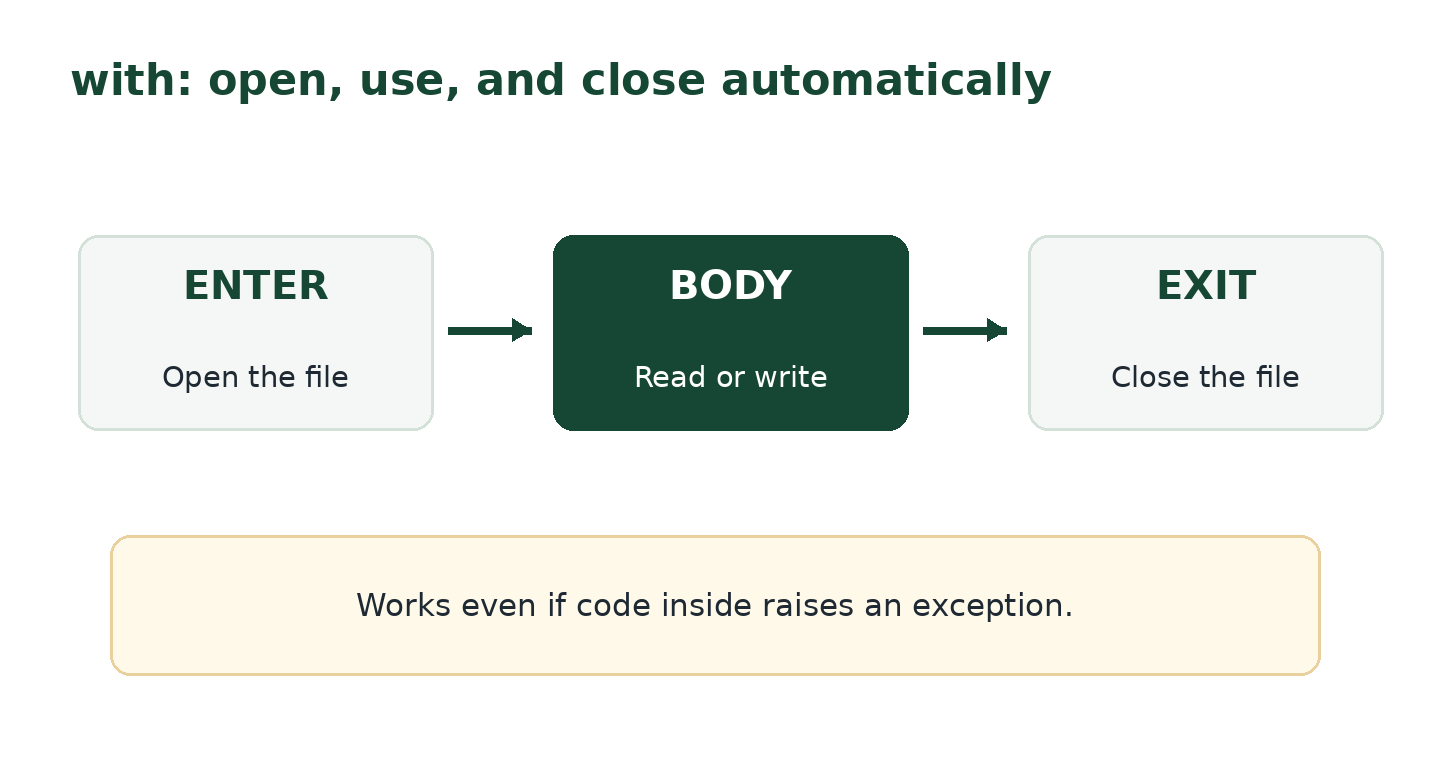
\includegraphics[width=0.78\linewidth,height=1.33in,keepaspectratio]{with-lifecycle.png}\end{center}
\begin{block}{Python / sample data}\begin{Verbatim}[fontsize=\scriptsize]
with open("message.txt", "r", encoding="utf-8") as f:
    text = f.read()

print(text)  # file is closed
\end{Verbatim}
\end{block}
\end{frame}
\begin{frame}[fragile]{Three ways to read text}
\begin{block}{Python / sample data}\begin{Verbatim}[fontsize=\scriptsize]
with open("notes.txt", encoding="utf-8") as f:
    all_text = f.read()

with open("notes.txt", encoding="utf-8") as f:
    first_line = f.readline()

with open("notes.txt", encoding="utf-8") as f:
    for line in f:
        print(line.rstrip("\n"))
\end{Verbatim}
\end{block}
\small\begin{itemize}
\item read(): all remaining text.
\item readline(): next line.
\item for line in f: process one line at a time.
\end{itemize}
\end{frame}
\begin{frame}[fragile]{What exactly is a line?}
\begin{block}{Python / sample data}\begin{Verbatim}[fontsize=\footnotesize]
line = "3.0 4.0\n"
print(repr(line))
print(line.strip())
parts = line.split()
print(parts)
print(float(parts[0]) + float(parts[1]))
\end{Verbatim}
\end{block}
\vspace{-0.07in}\begin{block}{Expected output}\begin{Verbatim}[fontsize=\scriptsize]
'3.0 4.0\n'
3.0 4.0
['3.0', '4.0']
7.0
\end{Verbatim}
\end{block}
\end{frame}
\begin{frame}[fragile]{Predict: what will print?}
\begin{block}{Python / sample data}\begin{Verbatim}[fontsize=\scriptsize]
with open("names.txt", "r", encoding="utf-8") as f:
    for line in f:
        print(line)

# names.txt contains two lines:
# Ada
# Lin
\end{Verbatim}
\end{block}
\small\begin{itemize}
\item Why might there be blank lines between printed names?
\item What would print(line.strip()) change?
\end{itemize}
\end{frame}
\begin{frame}[fragile]{File paths: where are we looking?}
\begin{block}{Python / sample data}\begin{Verbatim}[fontsize=\footnotesize]
from pathlib import Path

path = Path("data") / "message.txt"
print(path)           # data/message.txt (on Unix)
print(path.exists())  # True or False
print(Path.cwd())     # current working directory
\end{Verbatim}
\end{block}
\small\begin{itemize}
\item Relative paths start from the process working directory.
\item Path combines directory and filename without manually typing separators.
\end{itemize}
\end{frame}
\begin{frame}[fragile]{File modes in one picture}
\begin{columns}[T,onlytextwidth]\begin{column}{0.56\textwidth}\centering\lectureimage[2.1in]{open-modes.png}\end{column}\begin{column}{0.42\textwidth}
\small\begin{itemize}
\item Text mode is the default.
\item Modes change how opening affects the file.
\item Use only the minimum permission needed.
\end{itemize}
\end{column}\end{columns}
\end{frame}
\begin{frame}[fragile]{"w" versus "a": important distinction}
\begin{block}{Python / sample data}\begin{Verbatim}[fontsize=\footnotesize]
with open("log.txt", "w", encoding="utf-8") as f:
    f.write("First run\n")

with open("log.txt", "a", encoding="utf-8") as f:
    f.write("Second run\n")
\end{Verbatim}
\end{block}
\vspace{-0.07in}\begin{block}{Expected output}\begin{Verbatim}[fontsize=\scriptsize]
First run
Second run
\end{Verbatim}
\end{block}
\small\begin{itemize}
\item "w" creates or replaces contents.
\item "a" adds to the end. Neither adds a newline for you.
\end{itemize}
\end{frame}
\begin{frame}[fragile]{Other modes: x, b, and +}
\begin{itemize}
\item "x": create a new file; raise FileExistsError if it already exists.
\item "b": binary files; combine as "rb" or "wb" and work with bytes, not str.
\item "+": combine reading and writing, e.g., "r+"; rarely needed today.
\item For this course: start with "r", "w", "a", and with.
\end{itemize}
\vspace{0.1in}\begin{keyidea}\small Opening an existing file in "w" mode can destroy its previous contents.\end{keyidea}
\end{frame}
\begin{frame}[fragile]{Writing requires strings}
\begin{block}{Python / sample data}\begin{Verbatim}[fontsize=\footnotesize]
values = [7.0, 4.0, 5.0]
with open("sums.txt", "w", encoding="utf-8") as f:
    for number in values:
        f.write(str(number) + "\n")
\end{Verbatim}
\end{block}
\vspace{-0.07in}\begin{block}{Expected output}\begin{Verbatim}[fontsize=\scriptsize]
7.0
4.0
5.0
\end{Verbatim}
\end{block}
\small\begin{itemize}
\item write() writes the text you supply.
\item Convert numeric values to text and add \texttt{"\textbackslash{}n"} deliberately.
\end{itemize}
\end{frame}
\begin{frame}[fragile]{One pipeline: read, parse, compute, write}
\begin{block}{Python / sample data}\begin{Verbatim}[fontsize=\scriptsize]
results = []
with open("pairs.txt", encoding="utf-8") as source:
    for line in source:
        a, b = line.split()
        results.append(float(a) + float(b))

with open("sums.txt", "w", encoding="utf-8") as target:
    for value in results:
        target.write(f"{value}\n")
\end{Verbatim}
\end{block}
\small\begin{itemize}
\item Assume valid input today; next lecture considers malformed files.
\item Read once, process as Python data, then write.
\end{itemize}
\end{frame}
\begin{frame}[fragile]{Why plain split is not enough for CSV}
\begin{block}{Python / sample data}\begin{Verbatim}[fontsize=\footnotesize]
name,score
"Doe, Jane",93
Lin,87
\end{Verbatim}
\end{block}
\small\begin{itemize}
\item A comma can be part of a quoted field.
\item Using line.split(",") would incorrectly split "Doe, Jane".
\item The csv module knows the formatting rules.
\end{itemize}
\end{frame}
\begin{frame}[fragile]{CSV: reading rows}
\begin{center}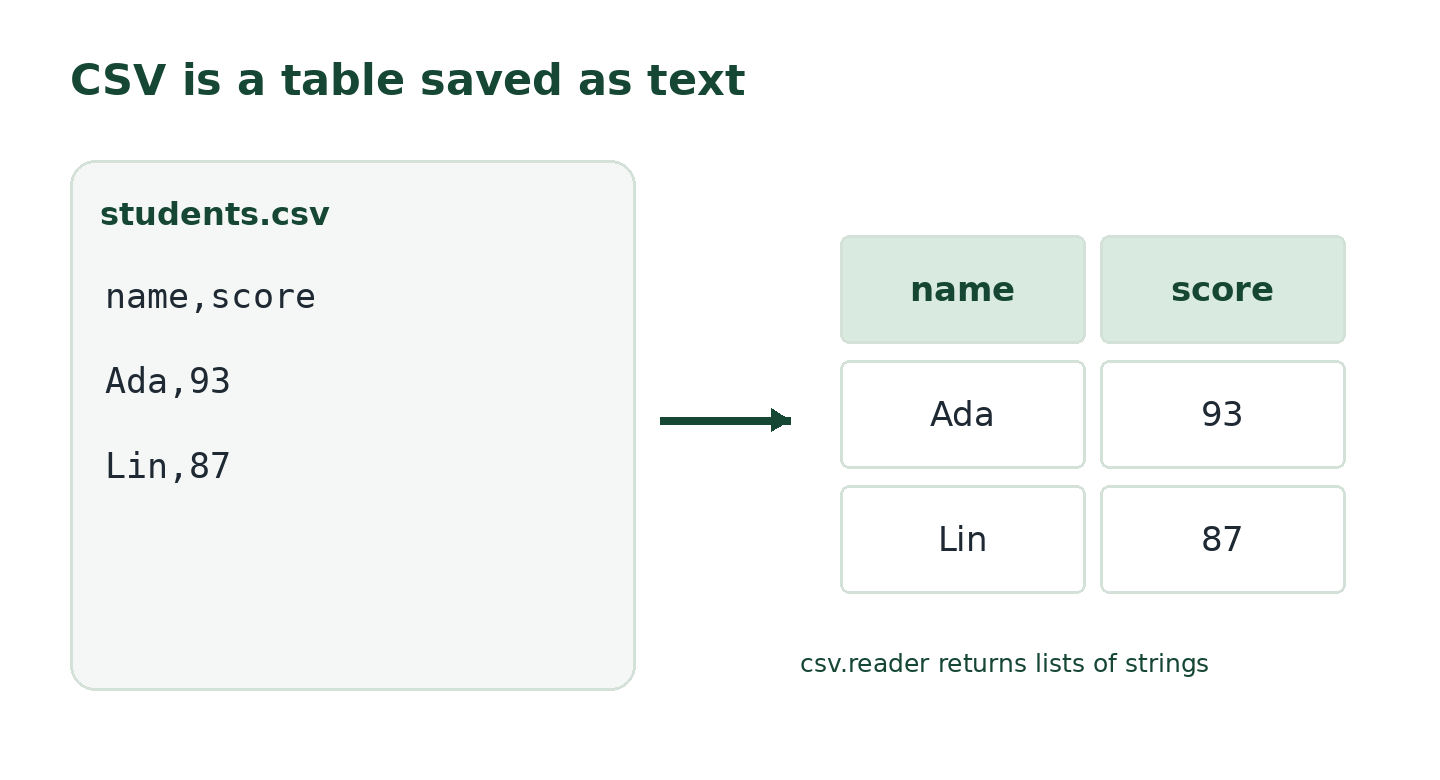
\includegraphics[width=0.78\linewidth,height=1.33in,keepaspectratio]{csv-row-map.png}\end{center}
\begin{block}{Python / sample data}\begin{Verbatim}[fontsize=\scriptsize]
import csv
with open("students.csv", newline="", encoding="utf-8") as f:
    for row in csv.reader(f):
        print(row)
\end{Verbatim}
\end{block}
\end{frame}
\begin{frame}[fragile]{CSV: use a header with DictReader}
\begin{block}{Python / sample data}\begin{Verbatim}[fontsize=\footnotesize]
import csv
with open("students.csv", newline="", encoding="utf-8") as f:
    for row in csv.DictReader(f):
        print(row["name"], int(row["score"]))
\end{Verbatim}
\end{block}
\small\begin{itemize}
\item Each row is a dict keyed by the header names.
\item Convert numeric fields: CSV initially holds text.
\item The parser handles quoted commas and row boundaries.
\end{itemize}
\end{frame}
\begin{frame}[fragile]{CSV: writing rows}
\begin{block}{Python / sample data}\begin{Verbatim}[fontsize=\footnotesize]
import csv
rows = [["name", "score"], ["Ada", 93], ["Lin", 87]]
with open("students.csv", "w", newline="",
          encoding="utf-8") as f:
    writer = csv.writer(f)
    writer.writerows(rows)
\end{Verbatim}
\end{block}
\small\begin{itemize}
\item The writer quotes fields when necessary.
\item newline="" avoids extra blank lines on some systems.
\end{itemize}
\end{frame}
\begin{frame}[fragile]{JSON: represent nested Python-like data}
\begin{columns}[T,onlytextwidth]\begin{column}{0.56\textwidth}\centering\lectureimage[2.1in]{json-structure.png}\end{column}\begin{column}{0.42\textwidth}
\small\begin{itemize}
\item JSON stores strings, numbers, booleans, null, arrays, and objects.
\item Python maps arrays to list, objects to dict, null to None.
\item The result is data, not Python source code.
\end{itemize}
\end{column}\end{columns}
\end{frame}
\begin{frame}[fragile]{Save and load a list using JSON}
\begin{block}{Python / sample data}\begin{Verbatim}[fontsize=\scriptsize]
import json
values = [3, 5, 8]

with open("values.json", "w", encoding="utf-8") as f:
    json.dump(values, f)

with open("values.json", "r", encoding="utf-8") as f:
    recovered = json.load(f)
print(recovered)   # [3, 5, 8]
\end{Verbatim}
\end{block}
\small\begin{itemize}
\item dump writes a JSON representation.
\item load parses JSON back into Python data.
\end{itemize}
\end{frame}
\begin{frame}[fragile]{Choose a representation intentionally}
\vspace{0.16in}\begin{center}\renewcommand{\arraystretch}{1.5}\begin{tabular}{p{0.19\linewidth}|p{0.42\linewidth}|p{0.29\linewidth}}\hline
\textbf{Format} & \textbf{Best for} & \textbf{Reading tool}\\\hline
Plain text & Human-readable lines & read / iteration\\\hline
CSV & Rows and columns & csv.reader\\\hline
JSON & Nested lists and dicts & json.load\\\hline
\end{tabular}\end{center}
\vspace{0.1in}\begin{keyidea}\small Avoid eval() on data read from files.\end{keyidea}
\end{frame}
\begin{frame}[fragile]{Quick choice: CSV or JSON?}
\begin{itemize}
\item A gradebook is naturally rows and columns: CSV.
\item A list of coordinates [x, y] pairs: JSON is convenient.
\item A configuration with nested options and lists: JSON.
\item A plain paragraph: simple text.
\end{itemize}
\vspace{0.1in}\begin{keyidea}\small Choosing a file format is choosing how to reconstruct the data later.\end{keyidea}
\end{frame}
\begin{frame}[fragile]{Can json.dump save a Student instance?}
\begin{block}{Python / sample data}\begin{Verbatim}[fontsize=\scriptsize]
class Student:
    def __init__(self, name: str, score: int):
        self.name = name
        self.score = score

student = Student("Ada", 93)
# json.dump(student, f)  # TypeError!
\end{Verbatim}
\end{block}
\small\begin{itemize}
\item A custom instance is not JSON-serializable by default.
\item Save its attributes in a supported representation.
\end{itemize}
\end{frame}
\begin{frame}[fragile]{Save attributes as a dictionary}
\begin{block}{Python / sample data}\begin{Verbatim}[fontsize=\footnotesize]
student = Student("Ada", 93)
record = {"name": student.name, "score": student.score}

with open("student.json", "w", encoding="utf-8") as f:
    json.dump(record, f, indent=2)
\end{Verbatim}
\end{block}
\vspace{-0.07in}\begin{block}{Expected output}\begin{Verbatim}[fontsize=\scriptsize]
{
  "name": "Ada",
  "score": 93
}
\end{Verbatim}
\end{block}
\end{frame}
\begin{frame}[fragile]{Reconstruct a new object}
\begin{block}{Python / sample data}\begin{Verbatim}[fontsize=\footnotesize]
with open("student.json", encoding="utf-8") as f:
    record = json.load(f)

restored = Student(record["name"], record["score"])
print(restored.name, restored.score)
\end{Verbatim}
\end{block}
\vspace{-0.07in}\begin{block}{Expected output}\begin{Verbatim}[fontsize=\scriptsize]
Ada 93
\end{Verbatim}
\end{block}
\small\begin{itemize}
\item Restored is a NEW Student instance.
\item The Python class code must be available.
\end{itemize}
\end{frame}
\begin{frame}[fragile]{Whole-list round trip}
\begin{columns}[T,onlytextwidth]\begin{column}{0.56\textwidth}\centering\lectureimage[2.1in]{object-roundtrip.png}\end{column}\begin{column}{0.42\textwidth}
\small\begin{itemize}
\item Turn each Student into a dict and save a list using json.dump.
\item Load the list of dicts with json.load.
\item Call Student(...) once for each saved record.
\end{itemize}
\end{column}\end{columns}
\end{frame}
\begin{frame}[fragile]{Small pattern worth remembering}
\begin{block}{Python / sample data}\begin{Verbatim}[fontsize=\scriptsize]
records = [{"name": s.name, "score": s.score}
           for s in students]

with open("students.json", "w", encoding="utf-8") as f:
    json.dump(records, f)

with open("students.json", encoding="utf-8") as f:
    rows = json.load(f)
students = [Student(r["name"], r["score"]) for r in rows]
\end{Verbatim}
\end{block}
\end{frame}
\begin{frame}[fragile]{The filesystem is a tree}
\begin{columns}[T,onlytextwidth]\begin{column}{0.56\textwidth}\centering\lectureimage[2.1in]{oswalk-tree.png}\end{column}\begin{column}{0.42\textwidth}
\small\begin{itemize}
\item Directories contain files and other directories.
\item Paths identify locations within the tree.
\item Tools can act on a single path or visit an entire subtree.
\end{itemize}
\end{column}\end{columns}
\end{frame}
\begin{frame}[fragile]{Create directories and empty files}
\begin{block}{Python / sample data}\begin{Verbatim}[fontsize=\scriptsize]
from pathlib import Path

folder = Path("output")
folder.mkdir(parents=True, exist_ok=True)

new_file = folder / "empty.txt"
new_file.touch(exist_ok=True)
\end{Verbatim}
\end{block}
\small\begin{itemize}
\item mkdir creates a directory.
\item touch creates an empty file if necessary.
\item Both methods have options that avoid errors when items exist.
\end{itemize}
\end{frame}
\begin{frame}[fragile]{Copy, move, and rename}
\begin{block}{Python / sample data}\begin{Verbatim}[fontsize=\footnotesize]
from pathlib import Path
import shutil

shutil.copy2("notes.txt", "backup.txt")
shutil.move("backup.txt", "archive/backup.txt")
Path("notes.txt").rename("renamed.txt")
\end{Verbatim}
\end{block}
\small\begin{itemize}
\item copy2 makes another file; the original remains.
\item move relocates a file (destination directory must exist).
\item rename changes a path, often used for renaming/moving.
\end{itemize}
\end{frame}
\begin{frame}[fragile]{Delete cautiously}
\begin{center}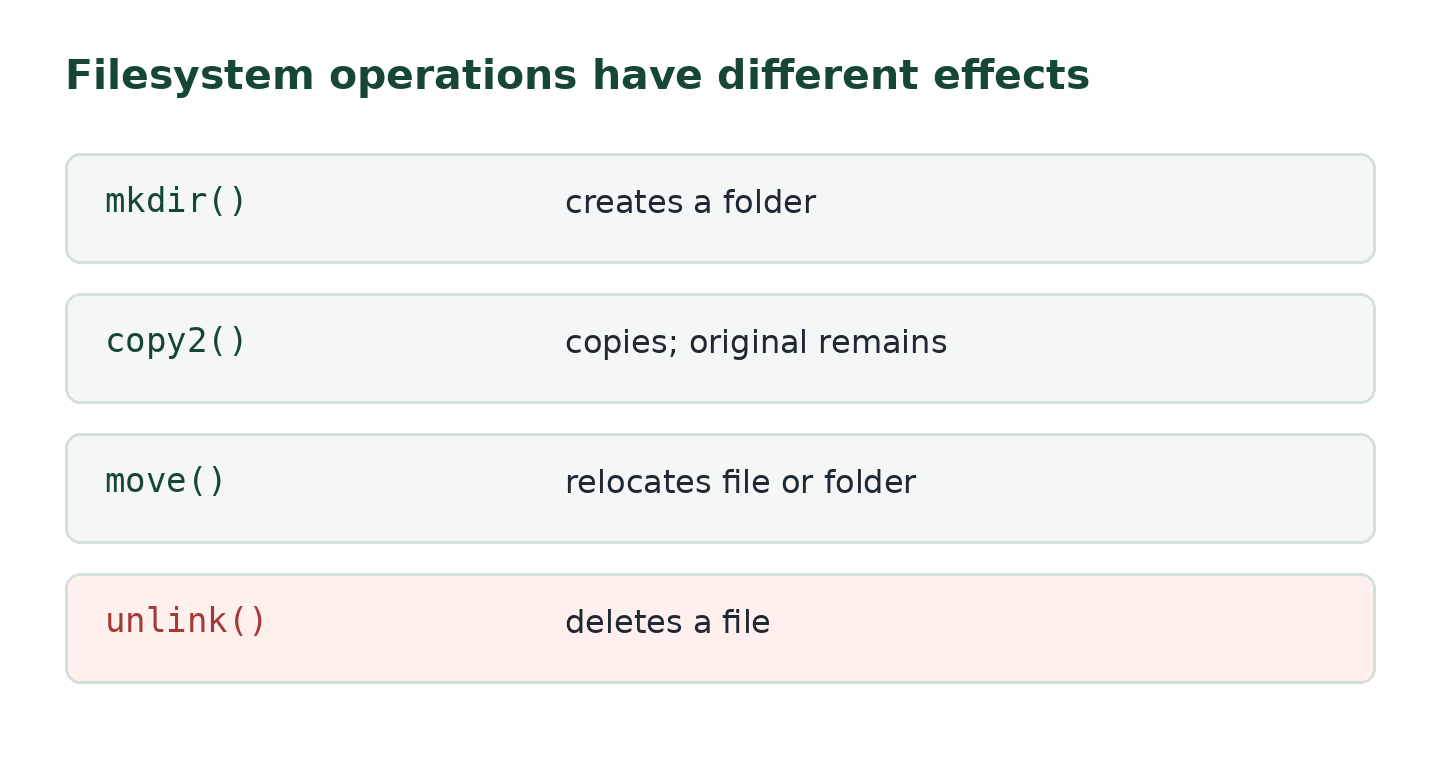
\includegraphics[width=0.78\linewidth,height=1.33in,keepaspectratio]{filesystem-ops.png}\end{center}
\begin{block}{Python / sample data}\begin{Verbatim}[fontsize=\scriptsize]
from pathlib import Path

target = Path("scratch.txt")
if target.is_file():
    target.unlink()  # deletes the file
\end{Verbatim}
\end{block}
\end{frame}
\begin{frame}[fragile]{Find files with os.walk}
\begin{block}{Python / sample data}\begin{Verbatim}[fontsize=\footnotesize]
import os

for root, dirs, files in os.walk("project"):
    print("folder:", root)
    for name in files:
        print("  file:", name)
\end{Verbatim}
\end{block}
\small\begin{itemize}
\item walk yields one (root, dirs, files) tuple per directory.
\item The traversal includes nested directories.
\end{itemize}
\end{frame}
\begin{frame}[fragile]{Search for matching filenames}
\begin{block}{Python / sample data}\begin{Verbatim}[fontsize=\scriptsize]
from pathlib import Path
import os

for root, dirs, files in os.walk("project"):
    for name in files:
        if name.endswith(".txt"):
            path = Path(root) / name
            print(path)
\end{Verbatim}
\end{block}
\small\begin{itemize}
\item Filename search does not inspect file contents.
\item Later, use with open(path) to search each matching file.
\end{itemize}
\end{frame}
\begin{frame}[fragile]{Predict: what paths will be reported?}
\begin{columns}[T,onlytextwidth]\begin{column}{0.56\textwidth}\centering\lectureimage[2.1in]{oswalk-tree.png}\end{column}\begin{column}{0.42\textwidth}
\small\begin{itemize}
\item Starting location: project/
\item Filter: filename ends with .txt
\item Predict the full paths printed.
\end{itemize}
\end{column}\end{columns}
\end{frame}
\begin{frame}[fragile]{Capstone: a misplaced encrypted note}
\begin{itemize}
\item One text file contains encrypted uppercase letters.
\item The sender used a Caesar shift, but the key was lost.
\item You suspect the plaintext contains the word BRIDGE.
\item Can we read the file, try possible keys, and find a plausible match?
\end{itemize}
\vspace{0.1in}\begin{keyidea}\small This is a search problem with only 26 possible keys.\end{keyidea}
\end{frame}
\begin{frame}[fragile]{A Caesar shift rotates letters}
\begin{columns}[T,onlytextwidth]\begin{column}{0.56\textwidth}\centering\lectureimage[2.1in]{caesar-shift.png}\end{column}\begin{column}{0.42\textwidth}
\small\begin{itemize}
\item Example encryption: BRIDGE becomes IYPKNL using shift +7.
\item To decrypt, shift backward by the candidate key.
\item Spaces and punctuation remain unchanged.
\end{itemize}
\end{column}\end{columns}
\end{frame}
\begin{frame}[fragile]{A helper to decode one letter}
\begin{block}{Python / sample data}\begin{Verbatim}[fontsize=\scriptsize]
def decode_caesar(text: str, key: int) -> str:
    result = ""
    for ch in text:
        if "A" <= ch <= "Z":
            position = ord(ch) - ord("A")
            result += chr((position - key) % 26 + ord("A"))
        else:
            result += ch
    return result
\end{Verbatim}
\end{block}
\small\begin{itemize}
\item Assume uppercase A-Z; keep nonletters.
\item \% 26 wraps around the alphabet.
\end{itemize}
\end{frame}
\begin{frame}[fragile]{Read the encrypted file}
\begin{block}{Python / sample data}\begin{Verbatim}[fontsize=\footnotesize]
with open("secret.txt", "r", encoding="utf-8") as f:
    ciphertext = f.read()

print(ciphertext)
\end{Verbatim}
\end{block}
\vspace{-0.07in}\begin{block}{Expected output}\begin{Verbatim}[fontsize=\scriptsize]
TLLA HA AOL VSK IYPKNL
\end{Verbatim}
\end{block}
\small\begin{itemize}
\item This came from MEET AT THE OLD BRIDGE using shift +7.
\item The program does not know the 7 yet.
\end{itemize}
\end{frame}
\begin{frame}[fragile]{Try every key: searching the key space}
\begin{block}{Python / sample data}\begin{Verbatim}[fontsize=\footnotesize]
for key in range(26):
    candidate = decode_caesar(ciphertext, key)
    if "BRIDGE" in candidate:
        print("Possible key:", key)
        print("Plaintext:", candidate)
\end{Verbatim}
\end{block}
\small\begin{itemize}
\item Use the decode function as a subroutine.
\item Search for the suspected word in each candidate.
\end{itemize}
\end{frame}
\begin{frame}[fragile]{Visualize the search}
\begin{columns}[T,onlytextwidth]\begin{column}{0.56\textwidth}\centering\lectureimage[2.1in]{caesar-key-search.png}\end{column}\begin{column}{0.42\textwidth}
\small\begin{itemize}
\item Most candidate keys produce unreadable results.
\item One candidate contains the suspected word.
\item A possible word is evidence, not mathematical proof.
\end{itemize}
\end{column}\end{columns}
\end{frame}
\begin{frame}[fragile]{Capstone solution: put the pieces together}
\begin{block}{Python / sample data}\begin{Verbatim}[fontsize=\scriptsize]
from pathlib import Path

path = Path("secret.txt")
with path.open("r", encoding="utf-8") as f:
    encrypted = f.read()

for key in range(26):
    message = decode_caesar(encrypted, key)
    if "BRIDGE" in message:
        print(key, message)
\end{Verbatim}
\end{block}
\vspace{-0.07in}\begin{block}{Expected output}\begin{Verbatim}[fontsize=\scriptsize]
7 MEET AT THE OLD BRIDGE
\end{Verbatim}
\end{block}
\small\begin{itemize}
\item File I/O -> strings -> reusable function -> search.
\item Extension: use os.walk to locate *.txt files first.
\end{itemize}
\end{frame}
\begin{frame}[fragile]{What could go wrong with the search?}
\begin{itemize}
\item Target may be absent even if a key is correct.
\item Short substrings can match by coincidence.
\item Different capitalization or punctuation can complicate matching.
\item Try more than one known word or inspect candidate sentences.
\end{itemize}
\vspace{0.1in}\begin{keyidea}\small Caesar ciphers are trivially breakable; never use them to protect real secrets.\end{keyidea}
\end{frame}
\begin{frame}[fragile]{One-minute exit ticket}
\begin{itemize}
\item Why is with open(...) preferred to manual close()?
\item Which open mode could overwrite an existing file?
\item When would you choose CSV instead of JSON?
\item What do you reconstruct after json.load returns a list of dicts?
\item How would you search every .txt file under a directory?
\end{itemize}
\vspace{0.1in}\begin{keyidea}\small Next: input validation and what to do when files or values are missing.\end{keyidea}
\end{frame}
\end{document}
